% Created by tikzDevice version 0.12.3.1 on 2021-08-27 10:42:22
% !TEX encoding = UTF-8 Unicode
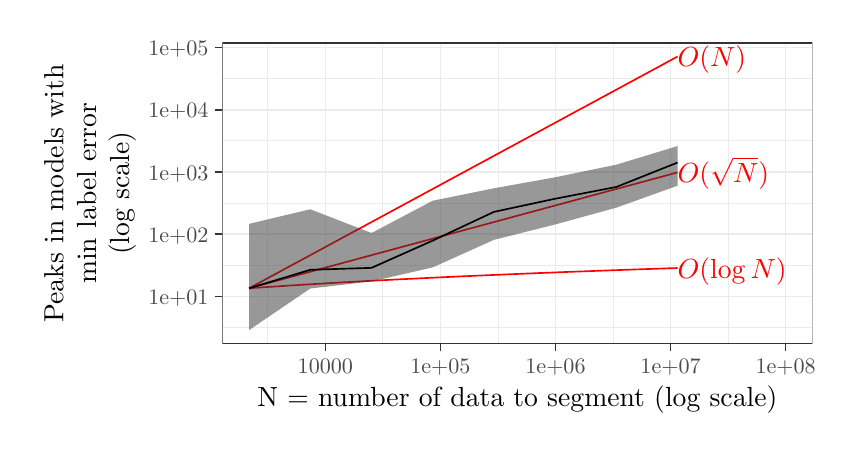
\begin{tikzpicture}[x=1pt,y=1pt]
\definecolor{fillColor}{RGB}{255,255,255}
\path[use as bounding box,fill=fillColor,fill opacity=0.00] (0,0) rectangle (289.08,144.54);
\begin{scope}
\path[clip] (  0.00,  0.00) rectangle (289.08,144.54);
\definecolor{drawColor}{RGB}{255,255,255}
\definecolor{fillColor}{RGB}{255,255,255}

\path[draw=drawColor,line width= 0.6pt,line join=round,line cap=round,fill=fillColor] (  0.00,  0.00) rectangle (289.08,144.54);
\end{scope}
\begin{scope}
\path[clip] ( 70.31, 30.33) rectangle (283.58,139.04);
\definecolor{fillColor}{RGB}{255,255,255}

\path[fill=fillColor] ( 70.31, 30.33) rectangle (283.58,139.04);
\definecolor{drawColor}{gray}{0.92}

\path[draw=drawColor,line width= 0.3pt,line join=round] ( 70.31, 36.20) --
	(283.58, 36.20);

\path[draw=drawColor,line width= 0.3pt,line join=round] ( 70.31, 58.68) --
	(283.58, 58.68);

\path[draw=drawColor,line width= 0.3pt,line join=round] ( 70.31, 81.17) --
	(283.58, 81.17);

\path[draw=drawColor,line width= 0.3pt,line join=round] ( 70.31,103.65) --
	(283.58,103.65);

\path[draw=drawColor,line width= 0.3pt,line join=round] ( 70.31,126.14) --
	(283.58,126.14);

\path[draw=drawColor,line width= 0.3pt,line join=round] ( 86.78, 30.33) --
	( 86.78,139.04);

\path[draw=drawColor,line width= 0.3pt,line join=round] (128.36, 30.33) --
	(128.36,139.04);

\path[draw=drawColor,line width= 0.3pt,line join=round] (169.94, 30.33) --
	(169.94,139.04);

\path[draw=drawColor,line width= 0.3pt,line join=round] (211.52, 30.33) --
	(211.52,139.04);

\path[draw=drawColor,line width= 0.3pt,line join=round] (253.10, 30.33) --
	(253.10,139.04);

\path[draw=drawColor,line width= 0.6pt,line join=round] ( 70.31, 47.44) --
	(283.58, 47.44);

\path[draw=drawColor,line width= 0.6pt,line join=round] ( 70.31, 69.93) --
	(283.58, 69.93);

\path[draw=drawColor,line width= 0.6pt,line join=round] ( 70.31, 92.41) --
	(283.58, 92.41);

\path[draw=drawColor,line width= 0.6pt,line join=round] ( 70.31,114.90) --
	(283.58,114.90);

\path[draw=drawColor,line width= 0.6pt,line join=round] ( 70.31,137.38) --
	(283.58,137.38);

\path[draw=drawColor,line width= 0.6pt,line join=round] (107.57, 30.33) --
	(107.57,139.04);

\path[draw=drawColor,line width= 0.6pt,line join=round] (149.15, 30.33) --
	(149.15,139.04);

\path[draw=drawColor,line width= 0.6pt,line join=round] (190.73, 30.33) --
	(190.73,139.04);

\path[draw=drawColor,line width= 0.6pt,line join=round] (232.31, 30.33) --
	(232.31,139.04);

\path[draw=drawColor,line width= 0.6pt,line join=round] (273.89, 30.33) --
	(273.89,139.04);
\definecolor{drawColor}{RGB}{255,0,0}

\path[draw=drawColor,line width= 0.6pt,line join=round] ( 80.01, 50.37) --
	( 81.57, 50.48) --
	( 83.13, 50.59) --
	( 84.70, 50.70) --
	( 86.26, 50.80) --
	( 87.82, 50.91) --
	( 89.39, 51.01) --
	( 90.95, 51.11) --
	( 92.52, 51.22) --
	( 94.08, 51.32) --
	( 95.64, 51.42) --
	( 97.21, 51.51) --
	( 98.77, 51.61) --
	(100.34, 51.71) --
	(101.90, 51.80) --
	(103.46, 51.90) --
	(105.03, 51.99) --
	(106.59, 52.08) --
	(108.16, 52.18) --
	(109.72, 52.27) --
	(111.28, 52.36) --
	(112.85, 52.45) --
	(114.41, 52.54) --
	(115.97, 52.62) --
	(117.54, 52.71) --
	(119.10, 52.80) --
	(120.67, 52.88) --
	(122.23, 52.97) --
	(123.79, 53.05) --
	(125.36, 53.13) --
	(126.92, 53.22) --
	(128.49, 53.30) --
	(130.05, 53.38) --
	(131.61, 53.46) --
	(133.18, 53.54) --
	(134.74, 53.62) --
	(136.31, 53.70) --
	(137.87, 53.78) --
	(139.43, 53.85) --
	(141.00, 53.93) --
	(142.56, 54.01) --
	(144.12, 54.08) --
	(145.69, 54.16) --
	(147.25, 54.23) --
	(148.82, 54.31) --
	(150.38, 54.38) --
	(151.94, 54.45) --
	(153.51, 54.52) --
	(155.07, 54.60) --
	(156.64, 54.67) --
	(158.20, 54.74) --
	(159.76, 54.81) --
	(161.33, 54.88) --
	(162.89, 54.95) --
	(164.46, 55.01) --
	(166.02, 55.08) --
	(167.58, 55.15) --
	(169.15, 55.22) --
	(170.71, 55.28) --
	(172.27, 55.35) --
	(173.84, 55.42) --
	(175.40, 55.48) --
	(176.97, 55.55) --
	(178.53, 55.61) --
	(180.09, 55.68) --
	(181.66, 55.74) --
	(183.22, 55.80) --
	(184.79, 55.87) --
	(186.35, 55.93) --
	(187.91, 55.99) --
	(189.48, 56.05) --
	(191.04, 56.11) --
	(192.61, 56.17) --
	(194.17, 56.24) --
	(195.73, 56.30) --
	(197.30, 56.36) --
	(198.86, 56.41) --
	(200.42, 56.47) --
	(201.99, 56.53) --
	(203.55, 56.59) --
	(205.12, 56.65) --
	(206.68, 56.71) --
	(208.24, 56.76) --
	(209.81, 56.82) --
	(211.37, 56.88) --
	(212.94, 56.93) --
	(214.50, 56.99) --
	(216.06, 57.05) --
	(217.63, 57.10) --
	(219.19, 57.16) --
	(220.76, 57.21) --
	(222.32, 57.27) --
	(223.88, 57.32) --
	(225.45, 57.37) --
	(227.01, 57.43) --
	(228.58, 57.48) --
	(230.14, 57.53) --
	(231.70, 57.59) --
	(233.27, 57.64) --
	(234.83, 57.69);

\path[draw=drawColor,line width= 0.6pt,line join=round] ( 80.01, 50.37) --
	( 81.57, 50.80) --
	( 83.13, 51.22) --
	( 84.70, 51.64) --
	( 86.26, 52.06) --
	( 87.82, 52.49) --
	( 89.39, 52.91) --
	( 90.95, 53.33) --
	( 92.52, 53.76) --
	( 94.08, 54.18) --
	( 95.64, 54.60) --
	( 97.21, 55.02) --
	( 98.77, 55.45) --
	(100.34, 55.87) --
	(101.90, 56.29) --
	(103.46, 56.72) --
	(105.03, 57.14) --
	(106.59, 57.56) --
	(108.16, 57.98) --
	(109.72, 58.41) --
	(111.28, 58.83) --
	(112.85, 59.25) --
	(114.41, 59.68) --
	(115.97, 60.10) --
	(117.54, 60.52) --
	(119.10, 60.94) --
	(120.67, 61.37) --
	(122.23, 61.79) --
	(123.79, 62.21) --
	(125.36, 62.64) --
	(126.92, 63.06) --
	(128.49, 63.48) --
	(130.05, 63.90) --
	(131.61, 64.33) --
	(133.18, 64.75) --
	(134.74, 65.17) --
	(136.31, 65.60) --
	(137.87, 66.02) --
	(139.43, 66.44) --
	(141.00, 66.86) --
	(142.56, 67.29) --
	(144.12, 67.71) --
	(145.69, 68.13) --
	(147.25, 68.56) --
	(148.82, 68.98) --
	(150.38, 69.40) --
	(151.94, 69.82) --
	(153.51, 70.25) --
	(155.07, 70.67) --
	(156.64, 71.09) --
	(158.20, 71.52) --
	(159.76, 71.94) --
	(161.33, 72.36) --
	(162.89, 72.78) --
	(164.46, 73.21) --
	(166.02, 73.63) --
	(167.58, 74.05) --
	(169.15, 74.48) --
	(170.71, 74.90) --
	(172.27, 75.32) --
	(173.84, 75.74) --
	(175.40, 76.17) --
	(176.97, 76.59) --
	(178.53, 77.01) --
	(180.09, 77.44) --
	(181.66, 77.86) --
	(183.22, 78.28) --
	(184.79, 78.70) --
	(186.35, 79.13) --
	(187.91, 79.55) --
	(189.48, 79.97) --
	(191.04, 80.40) --
	(192.61, 80.82) --
	(194.17, 81.24) --
	(195.73, 81.66) --
	(197.30, 82.09) --
	(198.86, 82.51) --
	(200.42, 82.93) --
	(201.99, 83.36) --
	(203.55, 83.78) --
	(205.12, 84.20) --
	(206.68, 84.62) --
	(208.24, 85.05) --
	(209.81, 85.47) --
	(211.37, 85.89) --
	(212.94, 86.32) --
	(214.50, 86.74) --
	(216.06, 87.16) --
	(217.63, 87.58) --
	(219.19, 88.01) --
	(220.76, 88.43) --
	(222.32, 88.85) --
	(223.88, 89.28) --
	(225.45, 89.70) --
	(227.01, 90.12) --
	(228.58, 90.54) --
	(230.14, 90.97) --
	(231.70, 91.39) --
	(233.27, 91.81) --
	(234.83, 92.24);

\path[draw=drawColor,line width= 0.6pt,line join=round] ( 80.01, 50.37) --
	( 81.57, 51.22) --
	( 83.13, 52.06) --
	( 84.70, 52.91) --
	( 86.26, 53.76) --
	( 87.82, 54.60) --
	( 89.39, 55.45) --
	( 90.95, 56.29) --
	( 92.52, 57.14) --
	( 94.08, 57.98) --
	( 95.64, 58.83) --
	( 97.21, 59.68) --
	( 98.77, 60.52) --
	(100.34, 61.37) --
	(101.90, 62.21) --
	(103.46, 63.06) --
	(105.03, 63.90) --
	(106.59, 64.75) --
	(108.16, 65.60) --
	(109.72, 66.44) --
	(111.28, 67.29) --
	(112.85, 68.13) --
	(114.41, 68.98) --
	(115.97, 69.82) --
	(117.54, 70.67) --
	(119.10, 71.52) --
	(120.67, 72.36) --
	(122.23, 73.21) --
	(123.79, 74.05) --
	(125.36, 74.90) --
	(126.92, 75.74) --
	(128.49, 76.59) --
	(130.05, 77.44) --
	(131.61, 78.28) --
	(133.18, 79.13) --
	(134.74, 79.97) --
	(136.31, 80.82) --
	(137.87, 81.66) --
	(139.43, 82.51) --
	(141.00, 83.36) --
	(142.56, 84.20) --
	(144.12, 85.05) --
	(145.69, 85.89) --
	(147.25, 86.74) --
	(148.82, 87.58) --
	(150.38, 88.43) --
	(151.94, 89.28) --
	(153.51, 90.12) --
	(155.07, 90.97) --
	(156.64, 91.81) --
	(158.20, 92.66) --
	(159.76, 93.50) --
	(161.33, 94.35) --
	(162.89, 95.20) --
	(164.46, 96.04) --
	(166.02, 96.89) --
	(167.58, 97.73) --
	(169.15, 98.58) --
	(170.71, 99.42) --
	(172.27,100.27) --
	(173.84,101.12) --
	(175.40,101.96) --
	(176.97,102.81) --
	(178.53,103.65) --
	(180.09,104.50) --
	(181.66,105.34) --
	(183.22,106.19) --
	(184.79,107.04) --
	(186.35,107.88) --
	(187.91,108.73) --
	(189.48,109.57) --
	(191.04,110.42) --
	(192.61,111.26) --
	(194.17,112.11) --
	(195.73,112.96) --
	(197.30,113.80) --
	(198.86,114.65) --
	(200.42,115.49) --
	(201.99,116.34) --
	(203.55,117.18) --
	(205.12,118.03) --
	(206.68,118.88) --
	(208.24,119.72) --
	(209.81,120.57) --
	(211.37,121.41) --
	(212.94,122.26) --
	(214.50,123.10) --
	(216.06,123.95) --
	(217.63,124.80) --
	(219.19,125.64) --
	(220.76,126.49) --
	(222.32,127.33) --
	(223.88,128.18) --
	(225.45,129.02) --
	(227.01,129.87) --
	(228.58,130.72) --
	(230.14,131.56) --
	(231.70,132.41) --
	(233.27,133.25) --
	(234.83,134.10);

\node[text=drawColor,anchor=base west,inner sep=0pt, outer sep=0pt, scale=  1.00] at (234.83,130.39) {$O(N)$};

\node[text=drawColor,anchor=base west,inner sep=0pt, outer sep=0pt, scale=  1.00] at (234.83, 53.98) {$O(\log N)$};

\node[text=drawColor,anchor=base west,inner sep=0pt, outer sep=0pt, scale=  1.00] at (234.83, 88.53) {$O(\sqrt N)$};
\definecolor{fillColor}{RGB}{51,51,51}

\path[fill=fillColor,fill opacity=0.50] ( 80.01, 73.65) --
	(102.12, 78.92) --
	(124.24, 70.34) --
	(146.36, 82.01) --
	(168.48, 86.50) --
	(190.59, 90.47) --
	(212.71, 95.03) --
	(234.83,101.75) --
	(234.83, 87.44) --
	(212.71, 79.50) --
	(190.59, 73.42) --
	(168.48, 67.87) --
	(146.36, 57.92) --
	(124.24, 52.84) --
	(102.12, 50.28) --
	( 80.01, 35.27) --
	cycle;

\path[] ( 80.01, 73.65) --
	(102.12, 78.92) --
	(124.24, 70.34) --
	(146.36, 82.01) --
	(168.48, 86.50) --
	(190.59, 90.47) --
	(212.71, 95.03) --
	(234.83,101.75);

\path[] (234.83, 87.44) --
	(212.71, 79.50) --
	(190.59, 73.42) --
	(168.48, 67.87) --
	(146.36, 57.92) --
	(124.24, 52.84) --
	(102.12, 50.28) --
	( 80.01, 35.27);
\definecolor{drawColor}{RGB}{0,0,0}

\path[draw=drawColor,line width= 0.6pt,line join=round] ( 80.01, 50.37) --
	(102.12, 57.05) --
	(124.24, 57.75) --
	(146.36, 67.59) --
	(168.48, 77.98) --
	(190.59, 82.72) --
	(212.71, 86.98) --
	(234.83, 95.80);
\definecolor{drawColor}{gray}{0.20}

\path[draw=drawColor,line width= 0.6pt,line join=round,line cap=round] ( 70.31, 30.33) rectangle (283.58,139.04);
\end{scope}
\begin{scope}
\path[clip] (  0.00,  0.00) rectangle (289.08,144.54);
\definecolor{drawColor}{gray}{0.30}

\node[text=drawColor,anchor=base east,inner sep=0pt, outer sep=0pt, scale=  0.80] at ( 65.36, 44.49) {1e+01};

\node[text=drawColor,anchor=base east,inner sep=0pt, outer sep=0pt, scale=  0.80] at ( 65.36, 66.97) {1e+02};

\node[text=drawColor,anchor=base east,inner sep=0pt, outer sep=0pt, scale=  0.80] at ( 65.36, 89.46) {1e+03};

\node[text=drawColor,anchor=base east,inner sep=0pt, outer sep=0pt, scale=  0.80] at ( 65.36,111.94) {1e+04};

\node[text=drawColor,anchor=base east,inner sep=0pt, outer sep=0pt, scale=  0.80] at ( 65.36,134.43) {1e+05};
\end{scope}
\begin{scope}
\path[clip] (  0.00,  0.00) rectangle (289.08,144.54);
\definecolor{drawColor}{gray}{0.20}

\path[draw=drawColor,line width= 0.6pt,line join=round] ( 67.56, 47.44) --
	( 70.31, 47.44);

\path[draw=drawColor,line width= 0.6pt,line join=round] ( 67.56, 69.93) --
	( 70.31, 69.93);

\path[draw=drawColor,line width= 0.6pt,line join=round] ( 67.56, 92.41) --
	( 70.31, 92.41);

\path[draw=drawColor,line width= 0.6pt,line join=round] ( 67.56,114.90) --
	( 70.31,114.90);

\path[draw=drawColor,line width= 0.6pt,line join=round] ( 67.56,137.38) --
	( 70.31,137.38);
\end{scope}
\begin{scope}
\path[clip] (  0.00,  0.00) rectangle (289.08,144.54);
\definecolor{drawColor}{gray}{0.20}

\path[draw=drawColor,line width= 0.6pt,line join=round] (107.57, 27.58) --
	(107.57, 30.33);

\path[draw=drawColor,line width= 0.6pt,line join=round] (149.15, 27.58) --
	(149.15, 30.33);

\path[draw=drawColor,line width= 0.6pt,line join=round] (190.73, 27.58) --
	(190.73, 30.33);

\path[draw=drawColor,line width= 0.6pt,line join=round] (232.31, 27.58) --
	(232.31, 30.33);

\path[draw=drawColor,line width= 0.6pt,line join=round] (273.89, 27.58) --
	(273.89, 30.33);
\end{scope}
\begin{scope}
\path[clip] (  0.00,  0.00) rectangle (289.08,144.54);
\definecolor{drawColor}{gray}{0.30}

\node[text=drawColor,anchor=base,inner sep=0pt, outer sep=0pt, scale=  0.80] at (107.57, 19.46) {10000};

\node[text=drawColor,anchor=base,inner sep=0pt, outer sep=0pt, scale=  0.80] at (149.15, 19.46) {1e+05};

\node[text=drawColor,anchor=base,inner sep=0pt, outer sep=0pt, scale=  0.80] at (190.73, 19.46) {1e+06};

\node[text=drawColor,anchor=base,inner sep=0pt, outer sep=0pt, scale=  0.80] at (232.31, 19.46) {1e+07};

\node[text=drawColor,anchor=base,inner sep=0pt, outer sep=0pt, scale=  0.80] at (273.89, 19.46) {1e+08};
\end{scope}
\begin{scope}
\path[clip] (  0.00,  0.00) rectangle (289.08,144.54);
\definecolor{drawColor}{RGB}{0,0,0}

\node[text=drawColor,anchor=base,inner sep=0pt, outer sep=0pt, scale=  1.00] at (176.95,  7.62) {N = number of data to segment (log scale)};
\end{scope}
\begin{scope}
\path[clip] (  0.00,  0.00) rectangle (289.08,144.54);
\definecolor{drawColor}{RGB}{0,0,0}

\node[text=drawColor,rotate= 90.00,anchor=base,inner sep=0pt, outer sep=0pt, scale=  1.00] at ( 12.89, 84.68) {Peaks in models with};

\node[text=drawColor,rotate= 90.00,anchor=base,inner sep=0pt, outer sep=0pt, scale=  1.00] at ( 24.77, 84.68) {min label error};

\node[text=drawColor,rotate= 90.00,anchor=base,inner sep=0pt, outer sep=0pt, scale=  1.00] at ( 36.65, 84.68) {(log scale)};
\end{scope}
\end{tikzpicture}
